\documentclass[11pt,a4paper]{article}
\usepackage[spanish,es-nodecimaldot]{babel}	% Utilizar español
\usepackage[utf8]{inputenc}					% Caracteres UTF-8
\usepackage{graphicx}						% Imagenes
\usepackage[hidelinks]{hyperref}			% Poner enlaces sin marcarlos en rojo
\usepackage{fancyhdr}						% Modificar encabezados y pies de pagina
\usepackage{float}							% Insertar figuras
\usepackage[textwidth=390pt]{geometry}		% Anchura de la pagina
\usepackage[nottoc]{tocbibind}				% Referencias (no incluir num pagina indice en Indice)
\usepackage{enumitem}						% Permitir enumerate con distintos simbolos
\usepackage[T1]{fontenc}					% Usar textsc en sections
\usepackage{amsmath}						% Símbolos matemáticos
\usepackage{listings}
\usepackage{color}

 
\definecolor{codegreen}{rgb}{0,0.6,0}
\definecolor{codegray}{rgb}{0.5,0.5,0.5}
\definecolor{codepurple}{rgb}{0.58,0,0.82}
\definecolor{backcolour}{rgb}{0.99,0.99,0.99}
 
\lstdefinestyle{mystyle}{
    backgroundcolor=\color{backcolour},   
    commentstyle=\color{codegreen},
    keywordstyle=\color{magenta},
    numberstyle=\tiny\color{codegray},
    stringstyle=\color{codepurple},
    basicstyle=\footnotesize,
    breakatwhitespace=false,         
    breaklines=true,                 
    captionpos=b,                    
    keepspaces=true,                 
    numbers=left,                    
    numbersep=5pt,                  
    showspaces=false,                
    showstringspaces=false,
    showtabs=false,                  
    tabsize=2
}
 
\lstset{style=mystyle, language=Java}

% Comando para poner el nombre de la asignatura
\newcommand{\asignatura}{Técnicas de los Sistemas Inteligentes}
\newcommand{\autor}{José María Sánchez Guerrero}
\newcommand{\titulo}{Práctica 1}
\newcommand{\subtitulo}{Desarrollo de un agente basado en búsqueda}

% Configuracion de encabezados y pies de pagina
\pagestyle{fancy}
\lhead{\autor{}}
\rhead{\asignatura{}}
\lfoot{Grado en Ingeniería Informática}
\cfoot{}
\rfoot{\thepage}
\renewcommand{\headrulewidth}{0.4pt}		% Linea cabeza de pagina
\renewcommand{\footrulewidth}{0.4pt}		% Linea pie de pagina

\begin{document}
\pagenumbering{gobble}

% Pagina de titulo
\begin{titlepage}

\begin{minipage}{\textwidth}

\centering

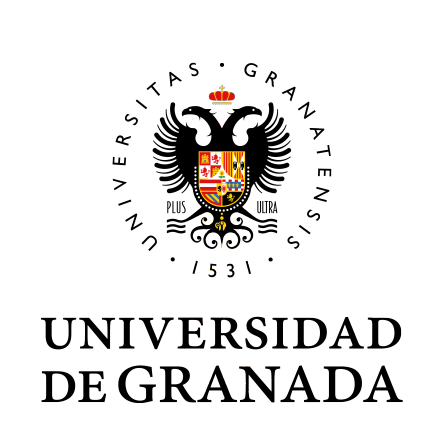
\includegraphics[scale=0.5]{img/ugr.png}\\

\textsc{\Large \asignatura{}\\[0.2cm]}
\textsc{GRADO EN INGENIERÍA INFORMÁTICA}\\[1cm]

\noindent\rule[-1ex]{\textwidth}{1pt}\\[1.5ex]
\textsc{{\Huge \titulo\\[0.5ex]}}
\textsc{{\Large \subtitulo\\}}
\noindent\rule[-1ex]{\textwidth}{2pt}\\[3.5ex]

\end{minipage}

\vspace{0.5cm}

\begin{minipage}{\textwidth}

\centering

\textbf{Autor}\\ {\autor{}}\\[2.5ex]
\textbf{Rama}\\ {Computación y Sistemas Inteligentes || Grupo 2 - Pablo Mesejo}\\[2.5ex]
\vspace{0.3cm}


\includegraphics[scale=0.3]{img/etsiit.jpeg}

\vspace{0.7cm}
\textsc{Escuela Técnica Superior de Ingenierías Informática y de Telecomunicación}\\
\vspace{1cm}
\textsc{Curso 2019-2020}
\end{minipage}
\end{titlepage}

\pagenumbering{arabic}
\tableofcontents
\thispagestyle{empty}				% No usar estilo en la pagina de indice

\newpage

\setlength{\parskip}{1em}
\setcounter{page}{1}


\section{Introducción}

La práctica consiste en implementar varios agentes que se puedan desenvolver adecuadamenete en los
distintos escenarios propuestos. Dispondremos de 5 mapas distintos, cada uno de ellos con un escenario
distinto.

\begin{itemize}
    \item En el primero simplemente tendremos que encontrar la salida
    \item En el segundo hay que recoger 10 gemas y luego salir
    \item En el tercero aguantar 2000 ticks del juego sin morir con un enemigo
    \item El cuarto aguantar 2000 ticks con varios enemigos
    \item El último será una fusión entre todos los otros, ya que hay que recoger 10 gemas y salir sin
          ser atrapado por ningun enemigo.
\end{itemize}

En mi caso he utilizado un algoritmo IDA* para encontrar los caminos más óptimos, y una técnica reactiva
que consiste en mantener al avatar lo más alejado posible de los enemigos en cada tick.


\section{Deliberativo}

Para nuestros agentes deliberativos vamos a utilizar, como hemos mencionado antes, el \textbf{algoritmo IDA*}.
He elegido este algoritmo porque está basado en el algoritmo base A* (es una extensión de este), sin embargo,
he decidido implementar IDA ya que obtiene los mismos resultados, pero no necesita almacenar todos y cada uno
de los posibles nodos candidatos. La gran ventaja que nos ofrece esto, es que reduce considerablemente el
consumo de memoria.

No obstante, pese a tener un consumo bajo en memoria, se podría haber implementado un algoritmo más eficiente
en cuanto a tiempo, sobre todo si tenemos en cuenta que disponemos 40 milisegundos por cada \textit{tick}. En
caso de que queramos calcular una ruta en este periodo de tiempo, puede ser que nos de error. En mi caso,
lo he dejado así porque los mapas son bastante pequeños y no muy complejos, por lo que no debería de tener
ningún problema; sin embargo, para mapas más difíciles sí que habría que mejorar su eficiencia.

A la hora de implementarlo, he necesitado dos clases. La primera es la clase ''\textbf{\textit{IDAStar.java}}'',
en la cual está implementado todo el algoritmo; y otra llamada ''\textbf{\textit{Node.java}}'', la cual
utilizamos para representar de una forma más sencilla cada una de las casillas del tablero adaptadas a nuestro
algoritmo. A continuación vamos a detallar cómo lo hemos hecho.

Empecemos con la clase \textbf{\textit{Node}} ya que la usaremos dentro de la otra. Lo primero es la declaración de
variables a utilizar:
\newline
\begin{lstlisting}
    // Valor heuristico del nodo actual
    private double hScore = Double.MIN_VALUE;
    // Coste del camino recorrido
    private double gScore = 0.0;
    // La suma de los valores anteriores
    private double fScore = 0.0;

    // Padre del nodo actual
    private Node parent;
    // Posicion en coordenadas (x,y) del nodo actual
    private Vector2d position;
\end{lstlisting}

Como es un algoritmo basado en el A*, tenemos que poner las 3 variables características de éste: $f()=g() + h()$.
Junto a ellas, también hay que poner la posición en coordenadas $(x,y)$ del nodo actual, y otra variable para
el padre, es decir, la posición de la cual se ha generado.

He añadido un constructor para poder crear un nuevo nodo a partir de una variable \textit{Vector2d}, que
representa una posición concreta en el mapa. Para acceder y modificar todas estas variables tendremos sus
correspondientes métodos \textit{getX()} y \textit{setX(value)}.

Implementaremos las siguientes funciones que nos podrán ser útiles en determinadas situaciones. Para comparar
un nodo con otro, es decir, comparar los valores de \textit{f()}, he añadido una función que devuelve -1, 1 o 0
dependiendo de si es menor, mayor o igual al nodo a comparar, respectivamente. Tenemos otra función que nos
dirá si un nodo es igual a otro (no en cuanto al valor de \textit{f()}, sino al estado de los nodos). Para
obtener los nodos sucesores del nodo actual, la cual inserta en una lista los nodos correspondientes a las
casillas que rodean a la actual, comprobando antes que esta casilla sea transitable, es decir, no sea un
obstaculo. Por último, tenemos la función que determina la \textit{h()}. Como estamos en un mapa cuadriculado,
la distancia al padre siempre va a ser 1 (excepto cuando hagamos un cambio de dirección que contará por 2).

Una vez hemos terminado con la clase \textit{Node}, vamos a pasar a la clase \textbf{\textit{IDAStar}}. En
ella tenemos las siguientes variables:
\begin{lstlisting}
    // Creamos las variables para los nodos

    // Nodo inicial desde donde saldra nuestro avatar
    private Node initialState;
    // Nodo objetivo para el camino
    private Node goalState;
    // Posiciones de los obstaculos del mapa
    private ArrayList<Vector2d> tiposObs;

\end{lstlisting}

Aqui también tenemos un constructor para que nos genere un camino a partir del nodo inicial, otro final y una
lista con las posiciones de los objetos por las que no puede pasar nuestro avatar.

La primera función más relevante de esta clase es \textbf{\textit{search()}}, en la cual comienza la
búsqueda. En ella realizaremos una búsqueda recursiva (que detallaremos posteriormente), hasta que la cota
hallada sea 0, o lo que es lo mismo, hasta que hayamos llegado al objetivo. Devuelve un $Node$ que es el
último nodo de la ruta óptima. Devolverá nulo si no se puede encontrar el nodo objetivo.

Ahora vamos a pasar a la función \textbf{\textit{recursive\_search()}}, la cual es la que maneja todo
el algoritmo y encuentra el camino óptimo desde dentro de la función \textit{search()}. Ésta busca recursivamente
los hijos de los nodos, evitando buscar el camino hacia abajo con una $f$ más alta que el límite $f$ actual.
Si se encuentran caminos con un limite más alto, devolverá la $f$ más pequeña sobre el límite encontrado.
Este límite sobre el $f$ mas pequeño es un nuevo límite $f$ potencial durante la próxima iteración. La función
devolverá 0 si se encuentra el nodo objetivo e Integer.MAX\_VALUE si no se puede encontrar el nodo objetivo.

Por último, tenemos una función \textit{\textbf{getPath()}} que devuelve una lista de nodos que representa el
camino óptimo. Como hemos mencionado, la función \textit{search()} sólo devuleve el nodo final, asi que esta
función se encargará de pasar por todos los padres del último nodo e insertalos en la lista, hasta llegar al
nulo.

Con esto ya hemos terminado de explicar las clases y funciones auxiliares que utilizaremos para los modelos
deliberativos, asi que pasemos a ver el funcionamiento de ambos.


\subsection{Deliberativo simple}

Antes de ejecutar el \textit{act} (en este y en todos los agentes), se inicializan las variables correspondientes
al factor de escala, posición del avatar, portal, objetos, muros, etc\dots; y en el caso del deliberativo, también
inicializamos y calculamos el path. Esto lo hacemos aquí, porque tenemos más margen de tiempo que en el \textit{act},
donde sólo tenemos 40 milisegundos para tomar una decisión.

La ventaja que tenemos en este agente deliberativo simple, es que no es necesario recalcular ningún path. Esto
quiere decir que el camino óptimo obtenido en un principio, nos servirá hasta el final.

Finalmente, lo único que tendremos que hacer en el \textit{act} es obtener el primer elemento del camino calculado
(siguiente posición del avatar), calcular el siguiente movimiento a partir de él y devolver su acción
correspondiente.


\subsection{Deliberativo compuesto}

En este agente procedemos de la misma forma que en el anterior, inicializando variables y calculando el camino
antes del \textit{act}. Lo que va a diferenciar a este agente es lo siguiente. Como tenemos que recoger una
serie de gemas antes, tenemos que obtener sus posiciones antes e ir metiendo los caminos a cada una de ellas en
el que tenemos actualmente.

Para ello calculamos el camino óptimo entre el avatar y la primera gema dada. Posteriormente, actualizamos
las posiciones del avatar, haciendo como que ya está en la primera gema; y de la gema, seleccionando la siguiente.
Con el código lo veremos más claro:
\newline
\begin{lstlisting}
    for (int i=0; i < posicionesGemas[0].size(); i++) {
        // Seleccionamos las gemas una a una
        gema = posicionesGemas[0].get(i).position;

        // Nuevo objetivo
        goalState = new Node(gema);
        
        // Se inicializa el objeto del pathfinder
        pf = new IDAStar(initialState, goalState, tiposObs);
        // Calculamos el camino
        ArrayList<Node> aux = pf.getPath( pf.search() );
        // Quitamos el primero, ya que estamos en el
        aux.remove(0);
        // Lo aniadimos al path completo
        path.addAll(aux);
        
        // Actualizamos la posicion
        initialState = goalState;
    }
\end{lstlisting}

Cuando no haya más gemas, ya pasaremos a seleccionar el portal como lo hacíamos en el deliberativo simple. Por
último, en el \textit{act}, volveremos a hacer lo mismo que antes, sacando de todo el camino calculado todas
las acciones correspondientes.




\newpage

\section{Reactivo}

Para implementar los agentes reactivos no se ha necesitado ninguna clase extra, por lo que estará todo en el
propio agente. Lo que hemos necesitado ha sido únicamente una función extra que estará implementada en los
propios agentes. Esta función se llama \textbf{\textit{simularAcciones(StateObservation)}}, y en la cual
determinaremos la acción más adecuada para alejarse del enemigo partiendo de las posiciones iniciales.

Para llevar esto a cabo, tomaremos todos los movimientos posibles y nos quedaremos con el que maximice la
distancia Manhattan entre el enemigo y el propio avatar. Esta es la parte del código que lo hace:
\newline
\begin{lstlisting}
    // Para todos los movimientos posibles
    for (Vector2d move : moves) {
    
        // Obtenemos la posicion del NPC
        Vector2d npcPosition = stateObs.getNPCPositions()[0].get(0).position;
    
        // Calculamos la distancia Manhattan
        double actualDistance = distManhattan(move, npcPosition);
        
        // Comprobamos si la actual es mayor que la mejor
        if (actualDistance > bestDistance) {
            bestDistance = actualDistance;
            bestMove = move;
        }
    }
\end{lstlisting}

A la hora de tomar todos los movimientos posibles, hay que tener en cuenta que algunos de ellos no los
podremos realizar, como por ejemplo, cuando estamos pegados a una pared, no podremos devolver la acción que
lleve al personaje hacia ella. Otra cosa que también tendremos que incluir en ellos es el movimiento
\textit{IDLE}, ya que en algunas ocasiones será mejor quedarse quieto a moverse.


\subsection{Reactivo simple}

En este agente no tendremos ningún problema con la función anteriormente explicada. Como no es muy lenta, en
cada tick de la ejecución podremos ejecutarla y que el avatar se mueva a la posición que mejor le venga,
maximizando la distancia con el único enemigo que hay.

En un principio, el avatar debería de irse a la esquina del mapa que esté más alejada de la zona en la que
se mueve el enemigo, y cuando éste se acerque se moverá hacia la dirección que más le convenga.


\subsection{Reactivo compuesto}

Al tener más de un enemigo, en este agente tendremos que hacer una modificacion en cuanto al anterior. Esta
modificación consiste en que, en la función \textit{simularAcciones()}, en vez de comprobar la distancia en
cuanto a un sólo enemigo, lo haremos para 2 o más.
\newline
\begin{lstlisting}
    // Mientras queden enemigos sin comprobar
    while( i < stateObs.getNPCPositions()[0].size() ) {
        npcPositions = stateObs.getNPCPositions()[0].get(i).position;
        actualDistance *= distManhattan( move, npcPositions );
        i++;
    } 

    // Hacemos la media geometrica
    actualDistance = Math.pow(actualDistance, 1.0 / 
                              stateObs.getNPCPositions()[0].size()); 
\end{lstlisting}


Como a la función le pasamos como parametro el estado de todo el mapa, podemos acceder a todas las posiciones
de todos los enemigos. Esto lo realizaremos para todos los movimientos posibles, y a la hora de comprobar la
ganancia entre uno y otro podemos comprobar que no hacemos una sumatoria y media normal y corriente, sino que
multiplicamos y luego hacemos la raíz cuadrada.

Esta es la \textbf{media geométrica}, y he decidido utilizar esta por el siguiente motivo. Si tenemos un enemigo
a 80 casillas de distancia y otro a 2, lo lógico sería moverse por el que tenemos cerca, no obstante, estos son
los resultados obtenidos:
$$aritmetica = (80+2)/2 = 40$$
$$geometrica = \sqrt{80+2} = 9.0553$$

La media geométrica es mucho más representativa en cuanto a lo cerca que está el enemigo que la aritmética, la
cual sigue diciendo que estamos bastante lejos de ellos. Por último, una vez obtenida esta distancia, sólo nos
queda comparar con el resto de movimientos y devolver el más adecuado.

Por otra parte, estos cálculos extra tampoco nos ocuparán mucho tiempo en el \textit{act}, asi que lo dejaremos
igual que estaba anteriormente.


\newpage

\section{Deliberativo-Reactivo}

Este agente es el más complejo de todos, no obstante, no incluiremos muchas cosas que no hayamos visto. Para
implementar este agente, hemos \textbf{unido el deliberativo compuesto y el reactivo compuesto}, de forma que en
el \textit{act} comprobamos primero si estamos lo suficientemente cerca del enemigo como para ejecutar el reactivo,
y en caso de no estarlo, pasar al deliberativo para coger las gemas e ir al portal.

Empezaremos inicializándolo todo como en el deliberativo compuesto y ejecutando. A continuación, cuando entremos
en el \textit{act}, lo primero será calcular la media geométrica de los enemigos como hicimos en el deliberativo
compuesto. Una vez hecho esto, tendremos que decidir.

En mi caso, tras hacer bastantes pruebas, he decidido que la distancia Manhattan mínima para ejecutar el reactivo
sea de 6 casillas. Si quisiéramos que nuestro avatar se arriesgue más, le bajaremos el valor; y en caso de que
queramos que sea más cautelosos, aumentaremos ese valor. (Línea 108 de la clase deliberativoReactivo.java en caso
de que se quiera modificar).

Como acabamos de decir, si baja de esta distancia se ejecutará el agente \textbf{reactivo}, el cual ya hemos explicado
cómo funciona. Además de esto, si se cumple la condición también borramos el camino óptimo que ya teníamos. Esto
lo hacemos porque el reactivo cambiará la posición del agente, y el camino que estábamos siguiendo será modificado.

Con esto pasamos a la parte del \textbf{deliberativo}, el cual ejecutaremos si estamos a una distancia lo
suficientemente alejada de los enemigos. En esta tenemos que volver a calcular un path, si ha sido limpiado por
el agente reactivo, y si no, vamos sacando las acciones correspondientes de este como ya explicamos previamente.
Junto a esto, he añadido una modificación que puede ayudar a nuestro agente a conseguir todas las gemas antes.
Consiste en que, si voy dirección a una gema y me encuentro a un enemigo, retrocederé. No obstante, al volver a
obtener las gemas con la función ''\textit{stateObs.getResourcesPositions()}'', las devolverá en el mismo orden que
antes y por tanto intentaremos coger la misma aunque el enemigo continúe ahí. Para solucionarlo he decidido hacer
un \textit{shuffle} del vector de gemas, y así obligarle a que vaya a por otra distinta.

En cuanto al rendimiento, 40 milisegundos puede resultar poco para todo lo que comprobamos, pero realmente no
suele tardar ni 5 milisegundos. Los únicos problemas llegarían si tenemos que recalcular una ruta muy compleja
dentro del \textit{act}, sin embargo, los mapas son bastante sencillos y no muy grandes, por lo que nunca
tendremos un error a causa de esto.

\end{document}